%% Synthetic test (1-station) 
\begin{figure}[h]
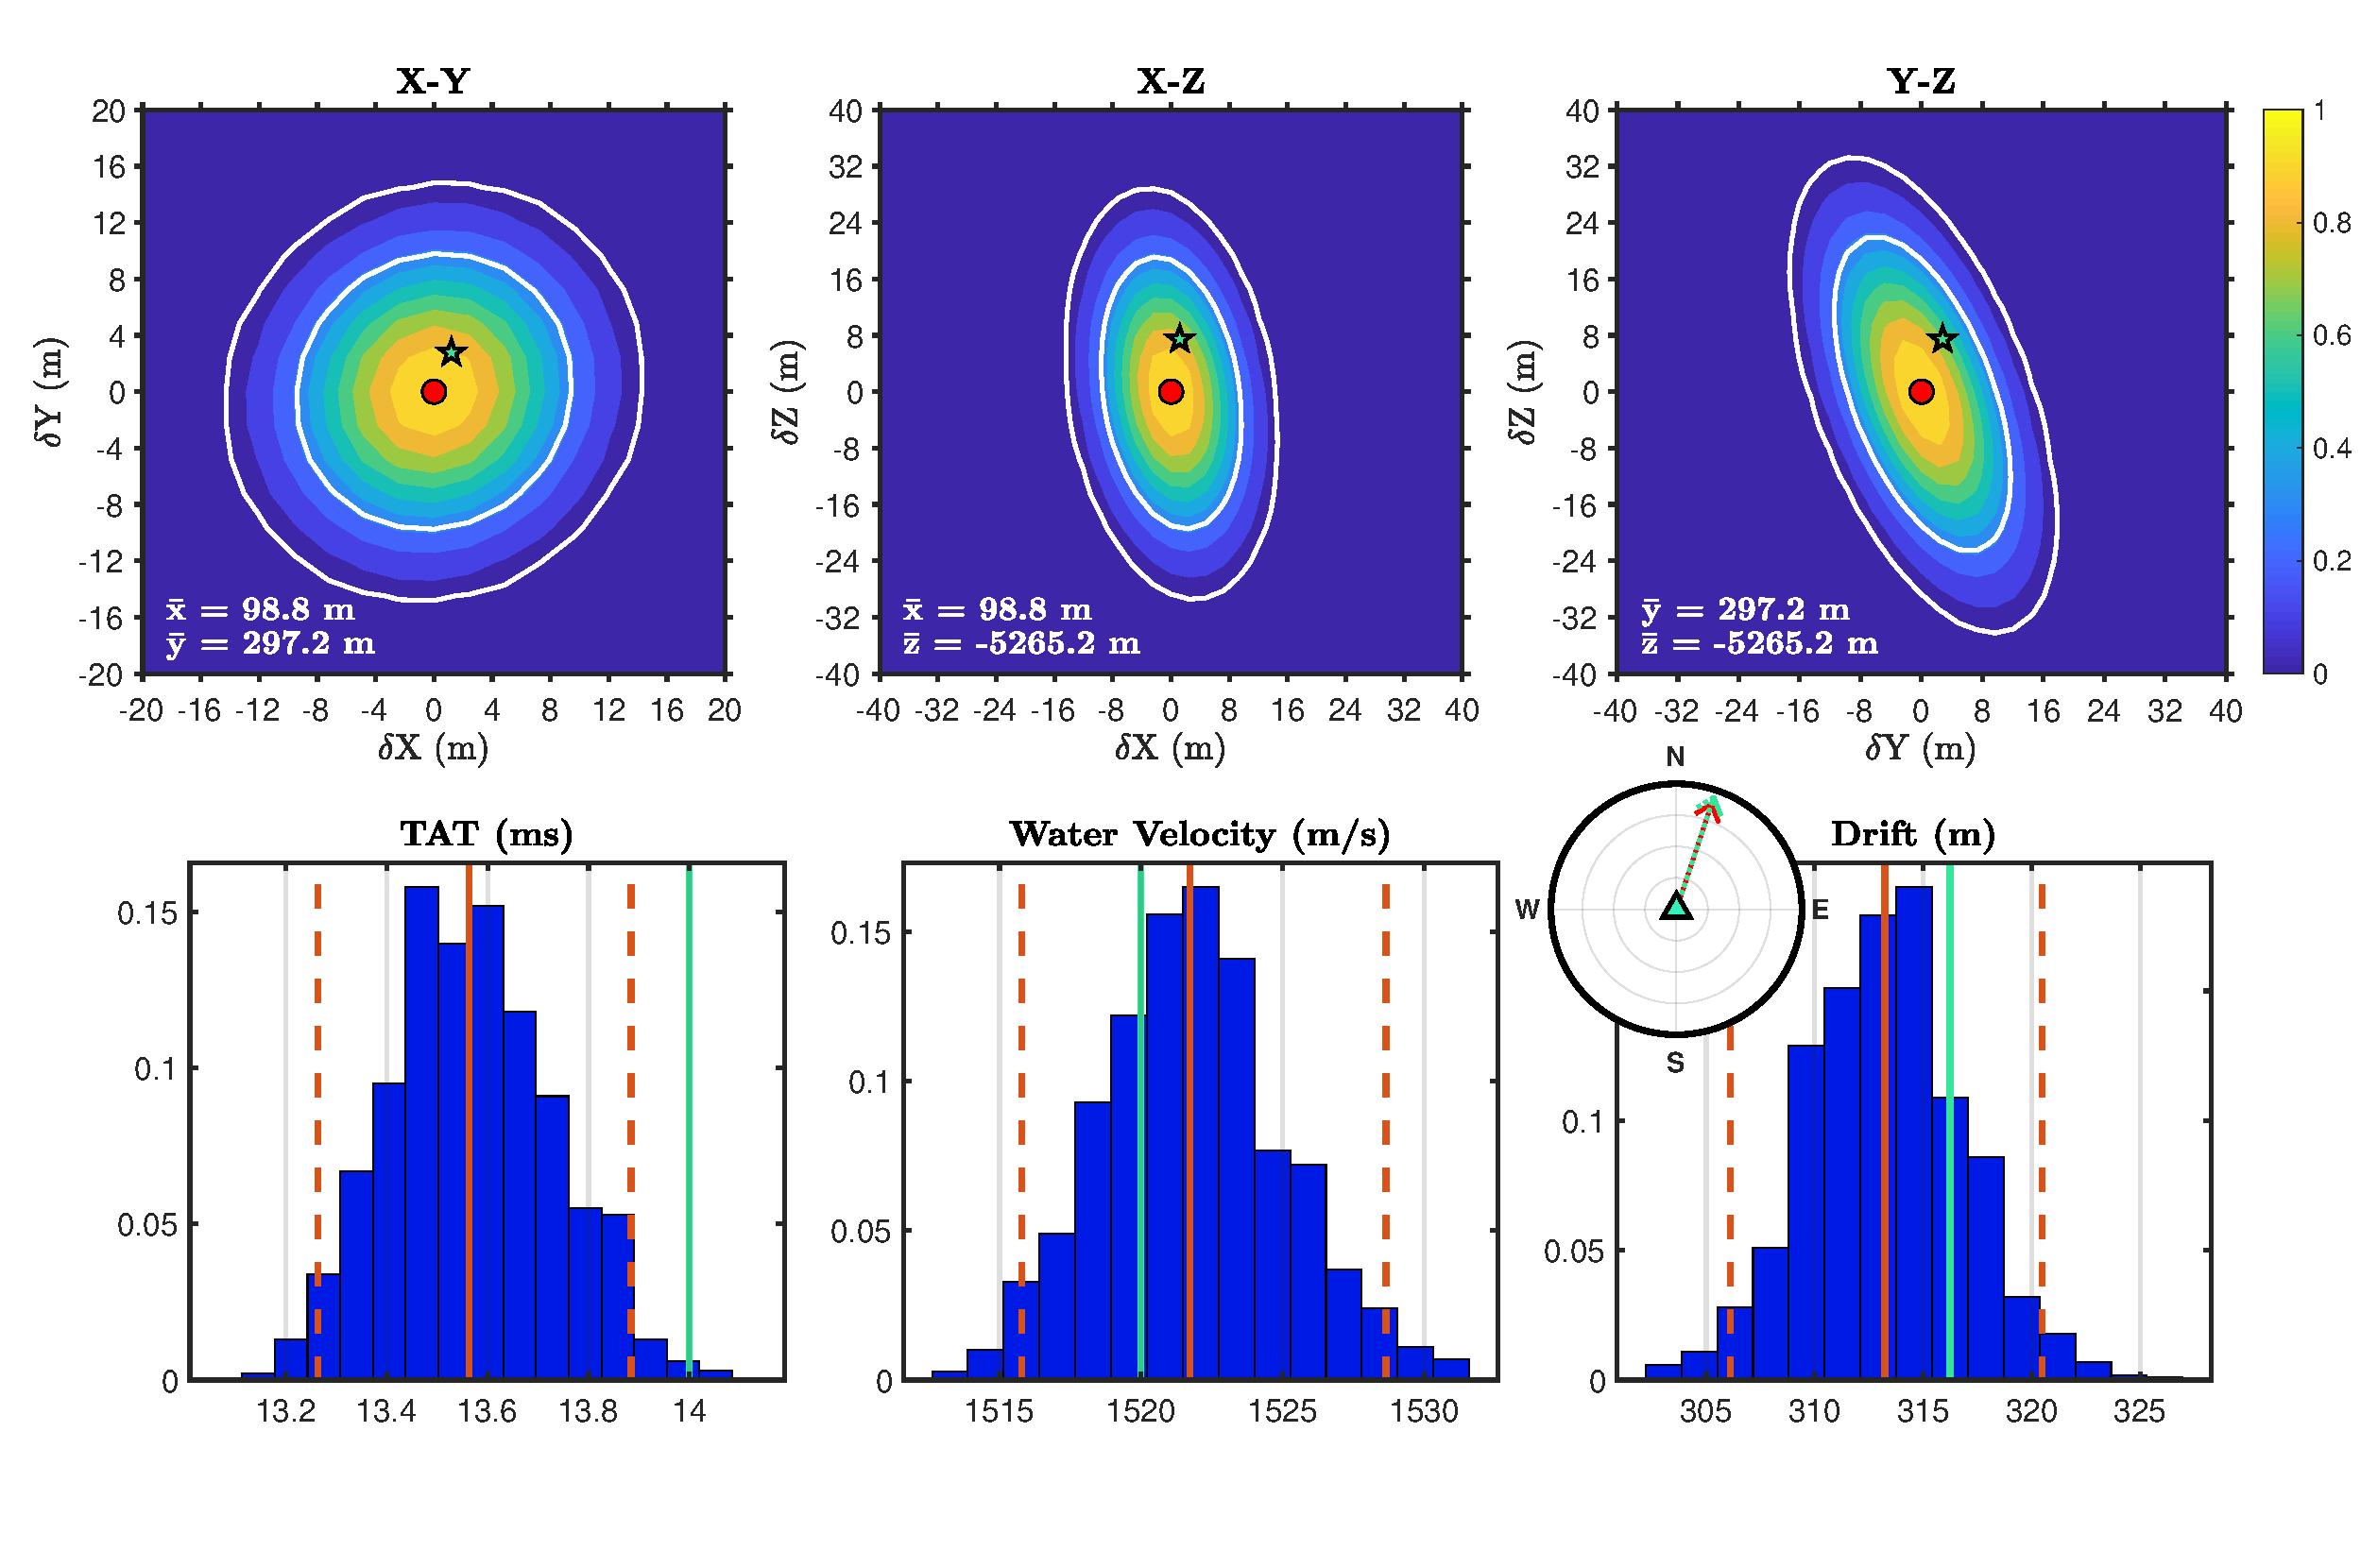
\includegraphics[trim=0cm 0cm 0cm 0cm,clip=true,width=\columnwidth]{Figure01.pdf}
\caption{Test of location algorithm using synthetic data. A comparison of the true input values (green star and lines) with the inverted model parameters (red circle and red solid lines) demonstrates that the location, depth, and water velocity are extremely well recovered, and the estimated uncertainties on these parameters are consonant with the actual misfit. Top three plots show slices through the F-test surface, contoured by probability. Bottom three plots show histograms from a bootstrap analysis with 95th percentile values indicated by dashed red lines. Inset shows the direction of true (green dashed) and estimated (red) drift with respect to the starting location. }
\label{fig:one_sta_synth}
\end{figure}

%% Example real station - survey pattern + residuals
\begin{figure}[h]
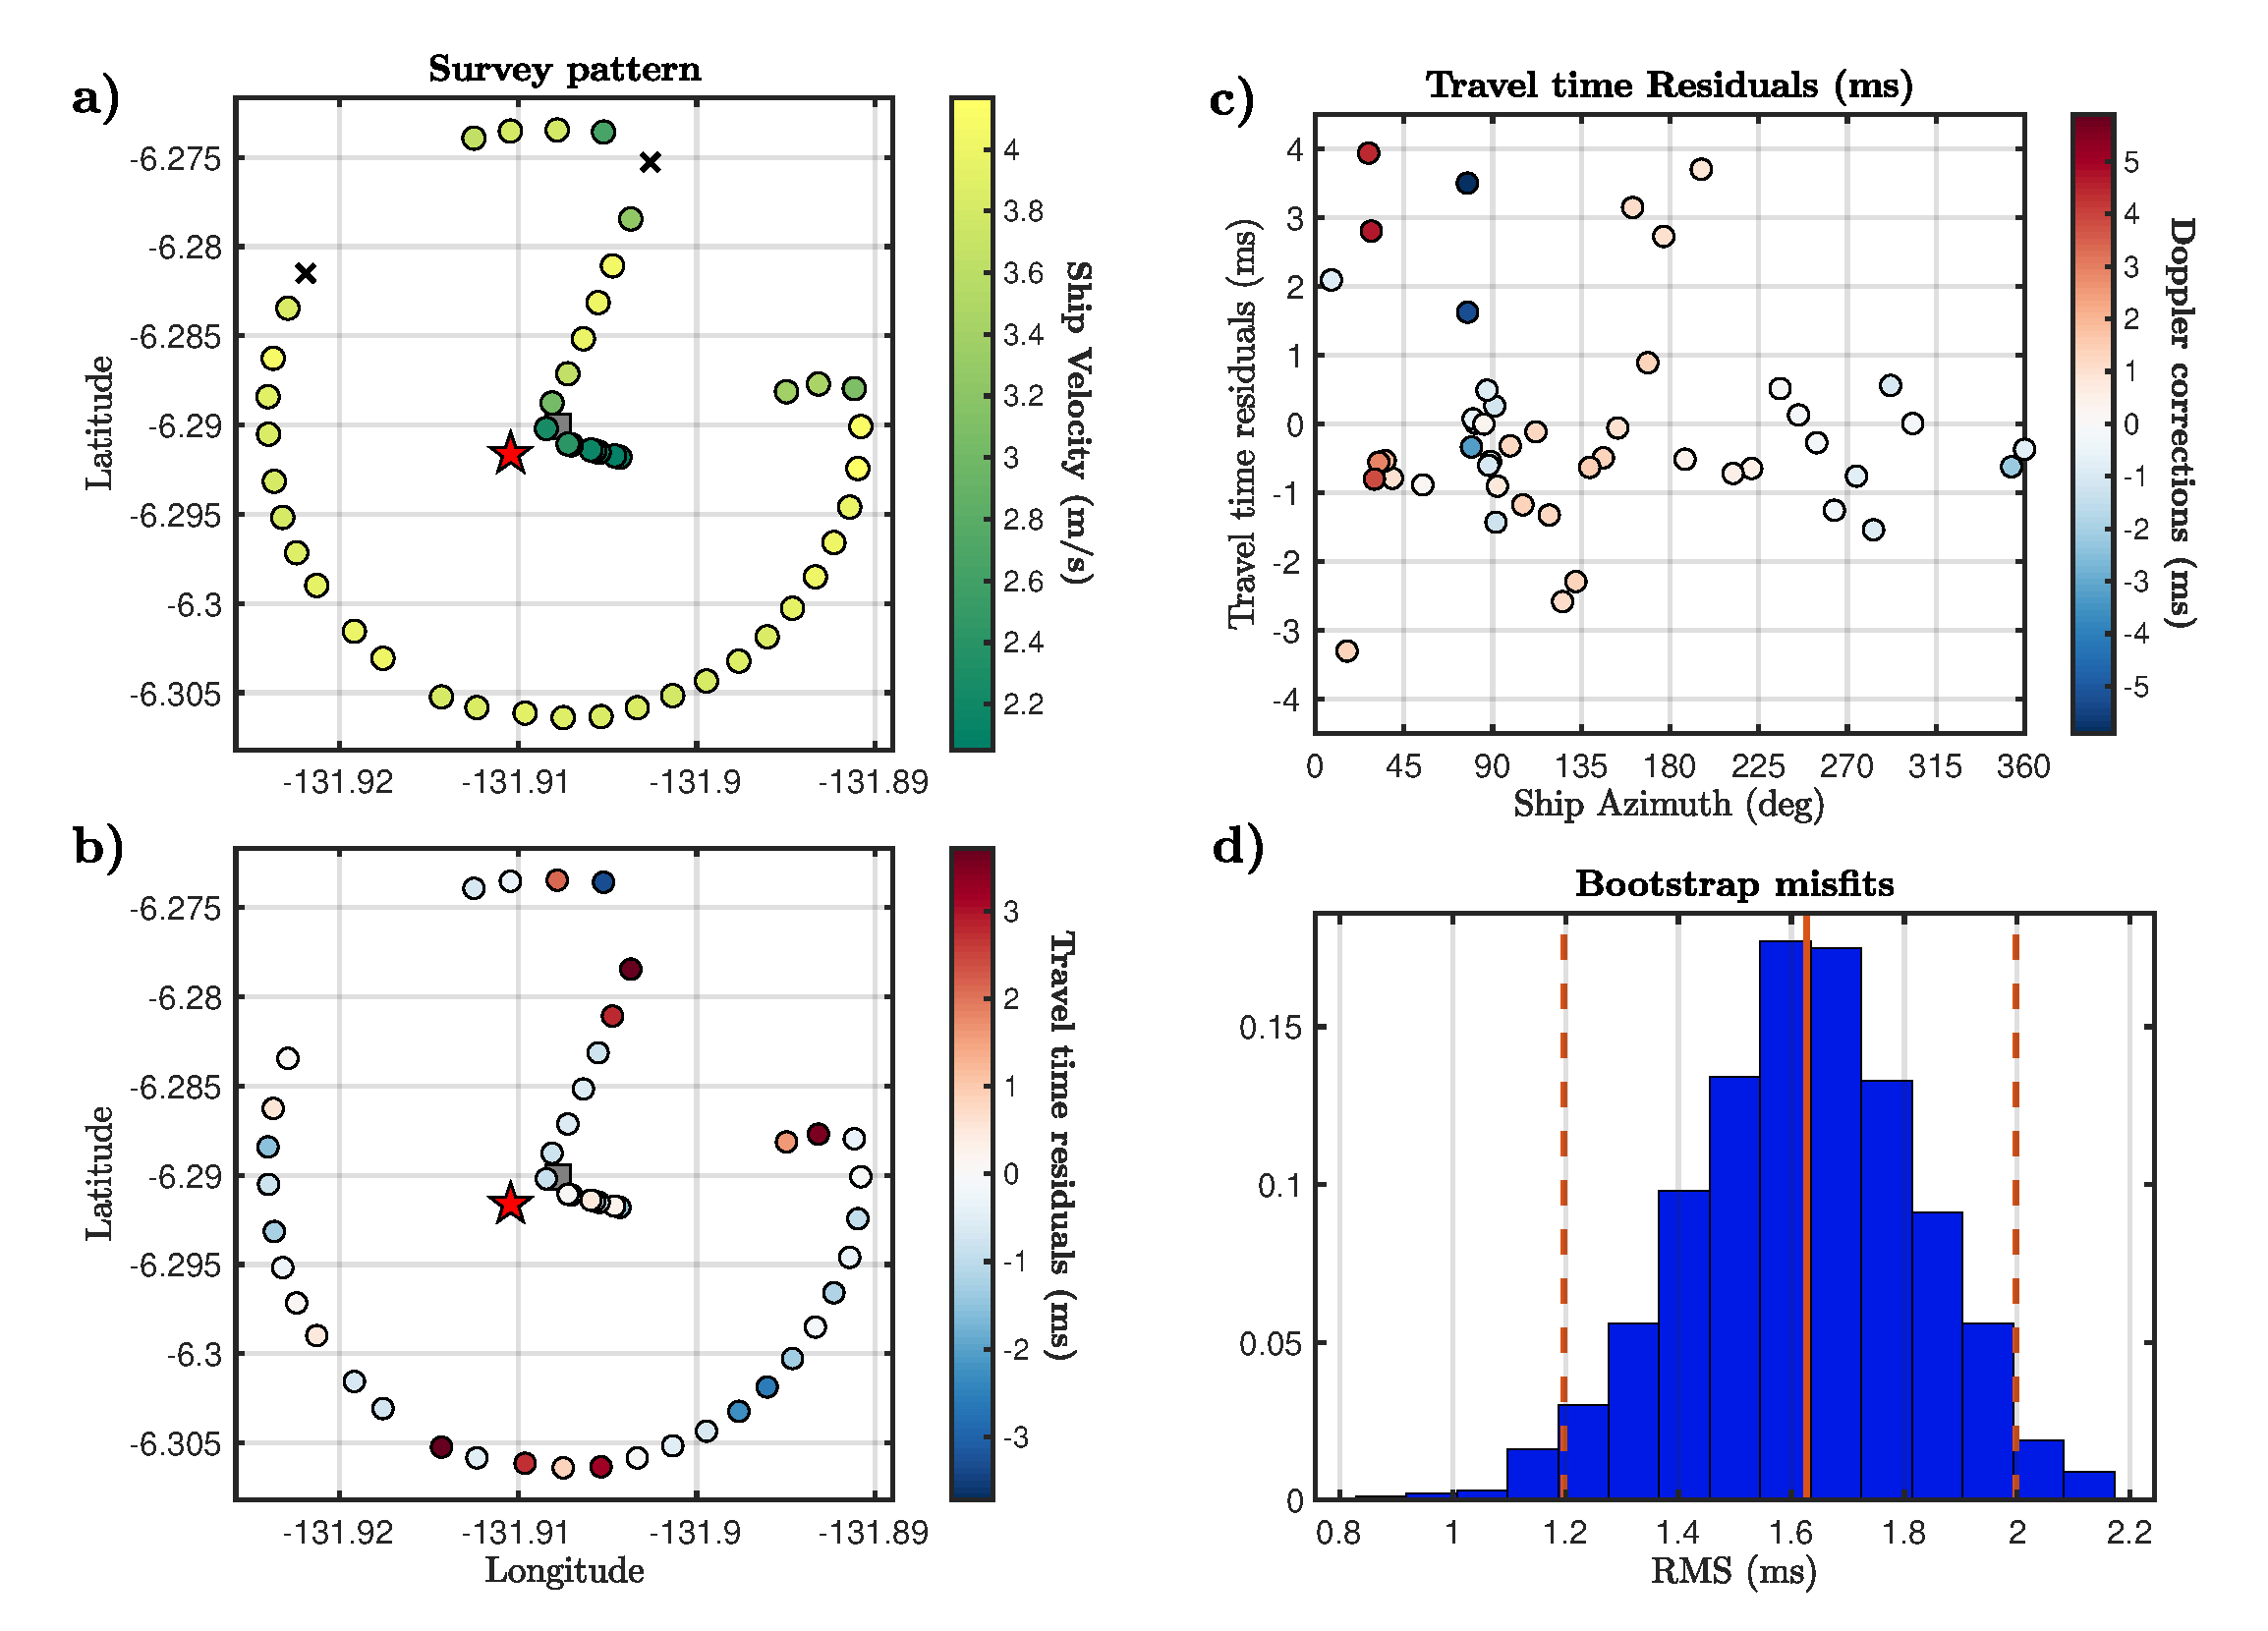
\includegraphics[trim=0cm 0cm 0cm 0cm,clip=true,width=\columnwidth]{Figure02.pdf}
\caption{Example inversion at station EC03 in the 2018 Young Pacific ORCA deployment. a) Map view of acoustic survey; colored circles are successful acoustic range measurements, black crosses are bad measurements rejected by automatic quality control, grey square is drop location, red star is final location. b) Map view of data residuals based on travel times computed using bootstrap mean station location. c) Data residuals plotted as a function of azimuth, colored by the computed doppler correction (not used in this inversion). d) Histogram of data RMS from the bootstrap; the RMS of the final model is shown as a red star.}
\label{fig:one_sta_real_survey}
\end{figure}

%% Example real station - bootstrap histogram
\begin{figure}[h]
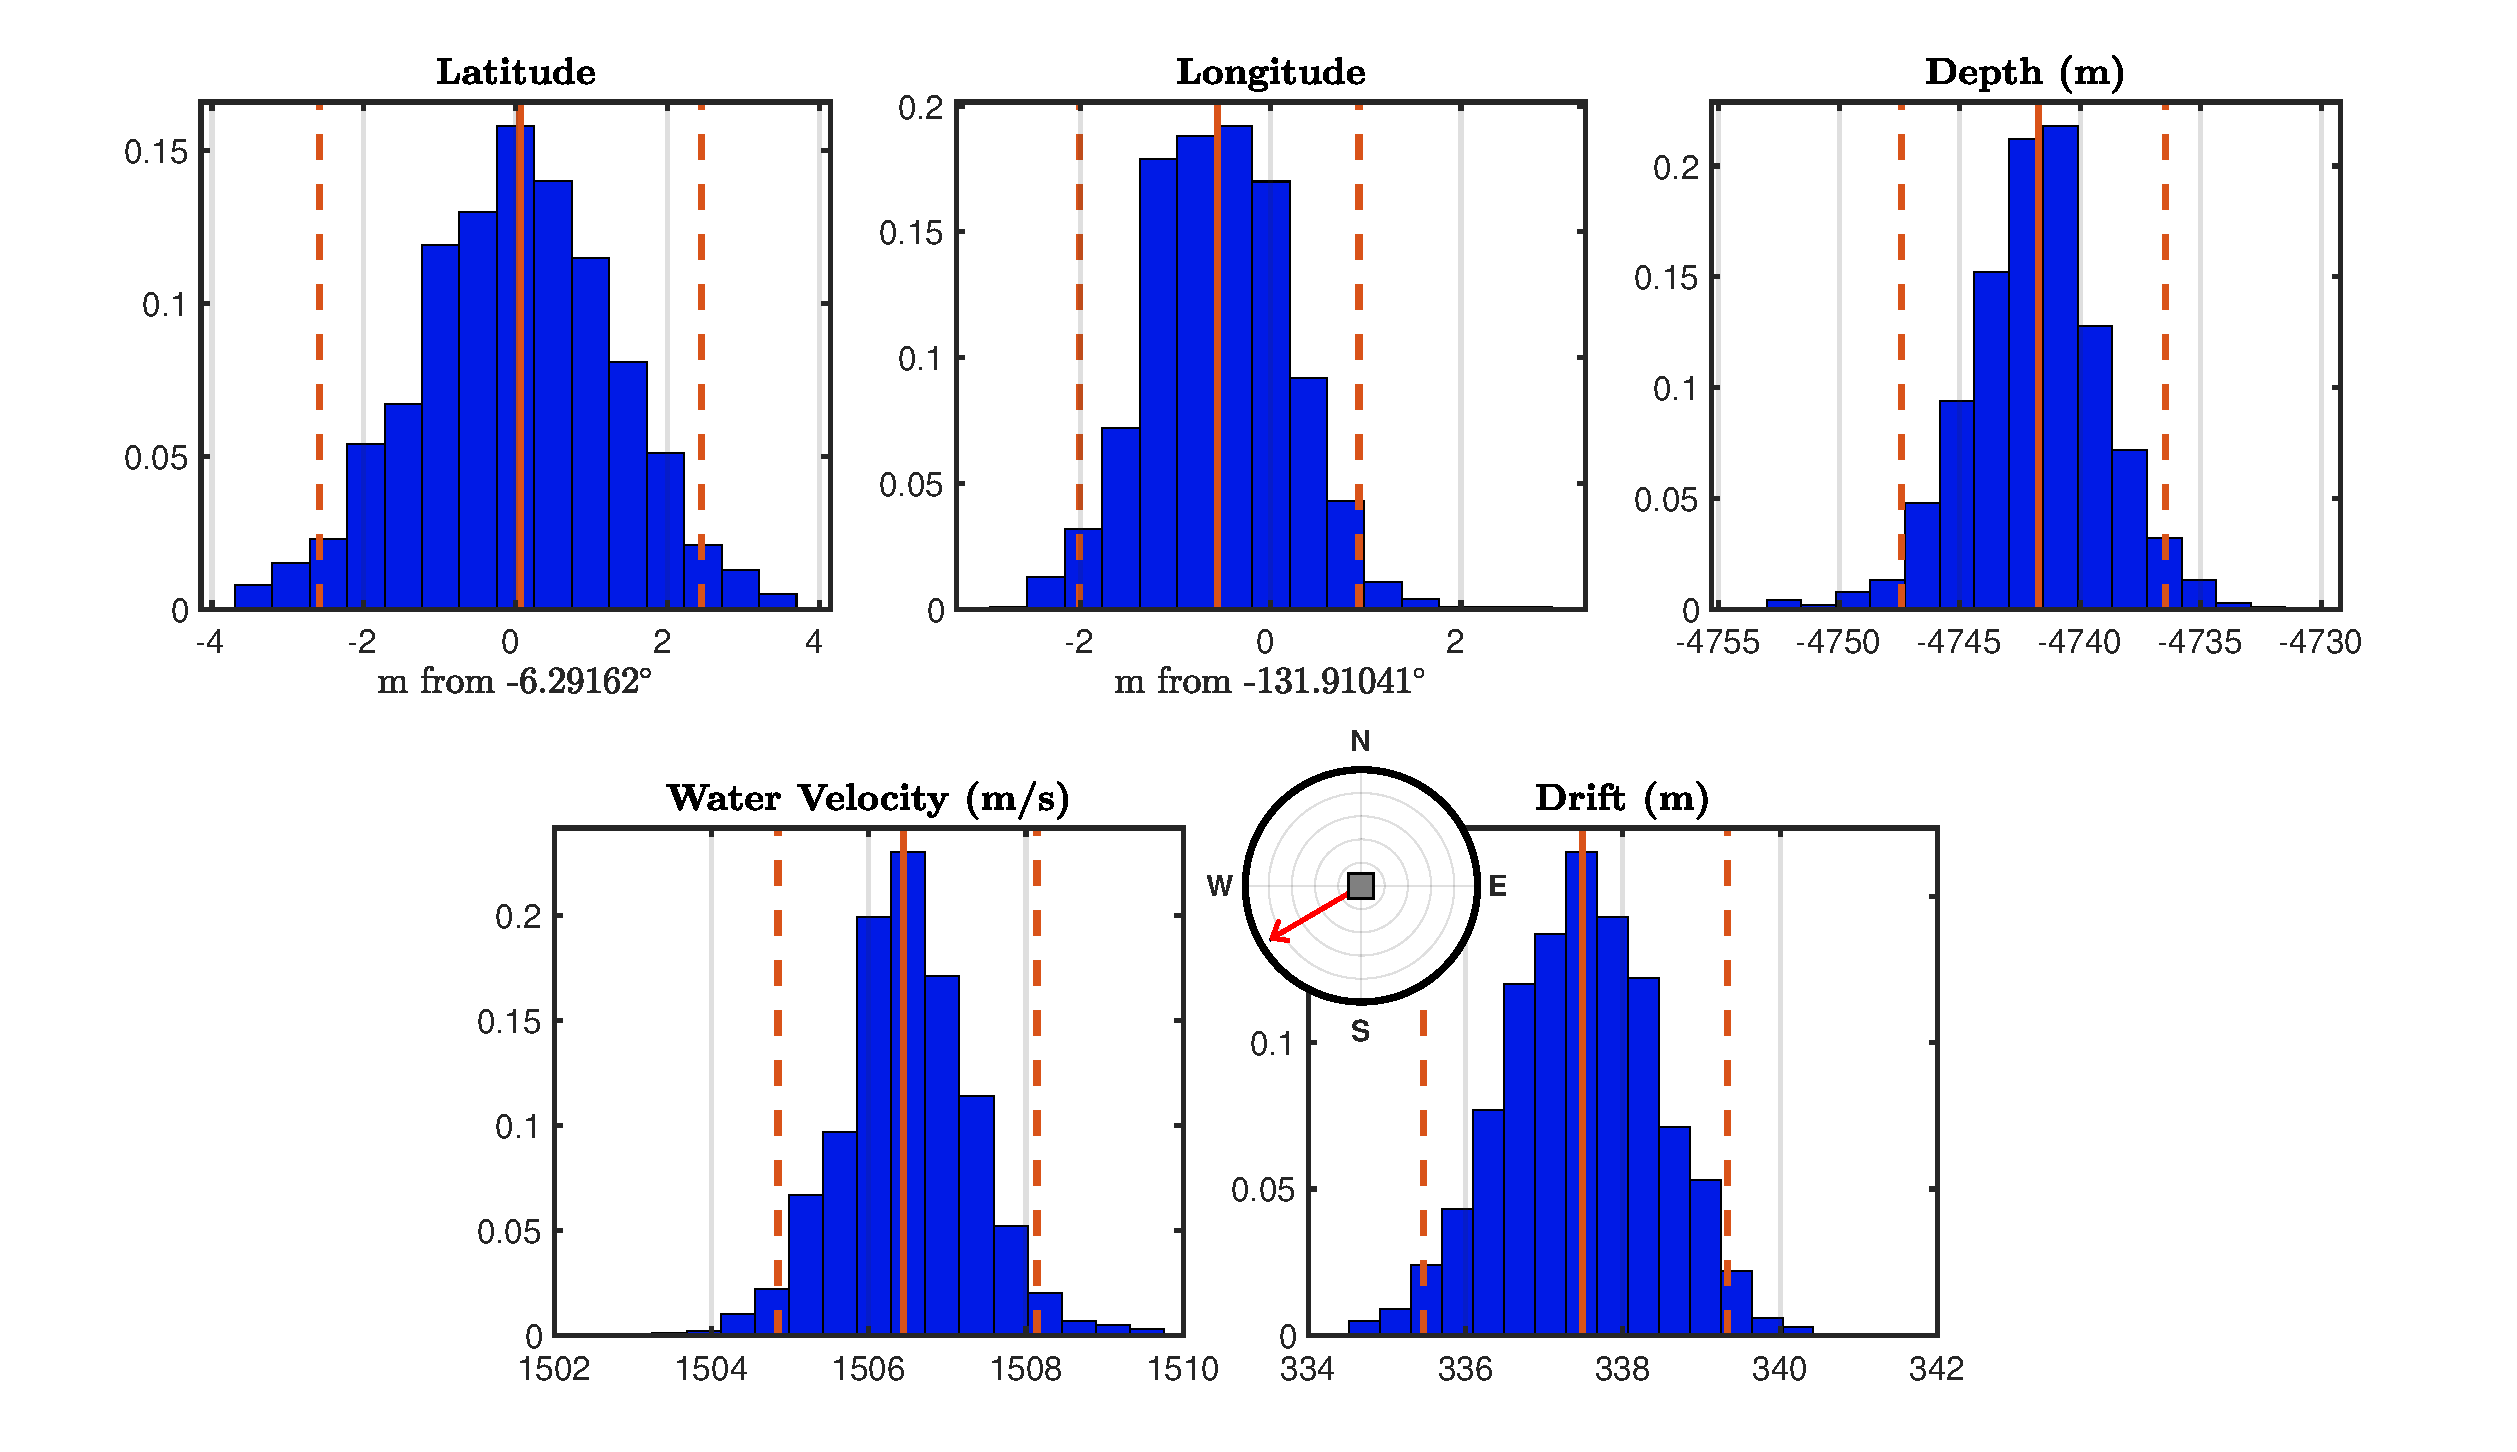
\includegraphics[trim=0cm 0cm 0cm 0cm,clip=true,width=\columnwidth]{Figure03.pdf}
\caption{Histograms of model parameters from the bootstrap inversion of station EC03 in the 2018 Young Pacific ORCA deployment. Red solid line shows mean value, while dashed lines indicate 95th percentiles. Latitude and longitude are plotted in meters from the mean point, for ease of interpretation. The inset plot shows the mean drift azimuth from the drop location (grey square).}
\label{fig:one_sta_real_histograms}
\end{figure}

%% Example real station - F-tests
\begin{figure}[h]
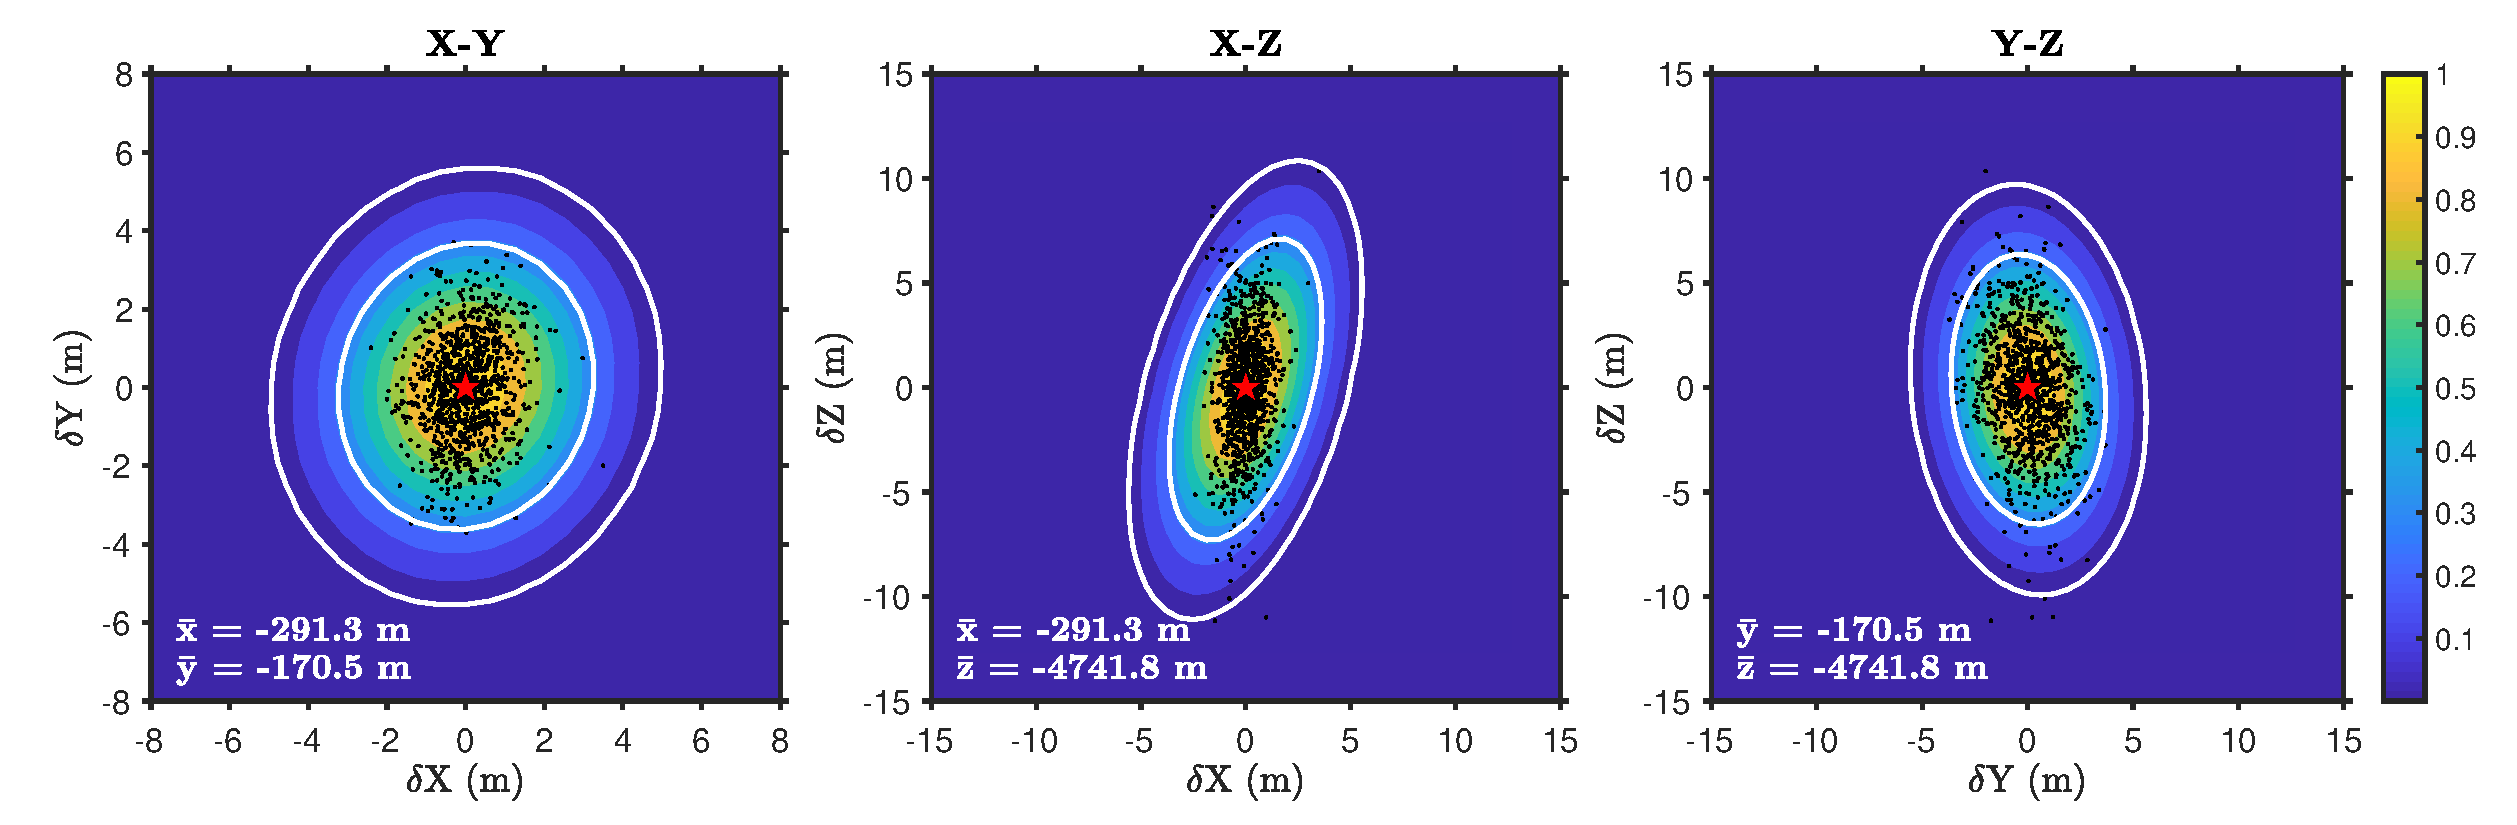
\includegraphics[trim=0cm 0cm 0cm 0cm,clip=true,width=\columnwidth]{Figure04.pdf}
\caption{ Three orthogonal slices through the F-test probability volume for station EC03 in the 2018 Young Pacific ORCA deployment, contoured by probability of true station location relative to the best fitting inverted location ($\bar{x},\bar{y},\bar{z}$), indicated by the red star. White contours show 68\% and 95\% contours. Black dots show individual locations from the bootstrap analysis (Figure \ref{fig:one_sta_real_histograms}). }
\label{fig:one_sta_real_ftests}
\end{figure}


%%% All stations meso eddy
%\begin{figure}[h]
%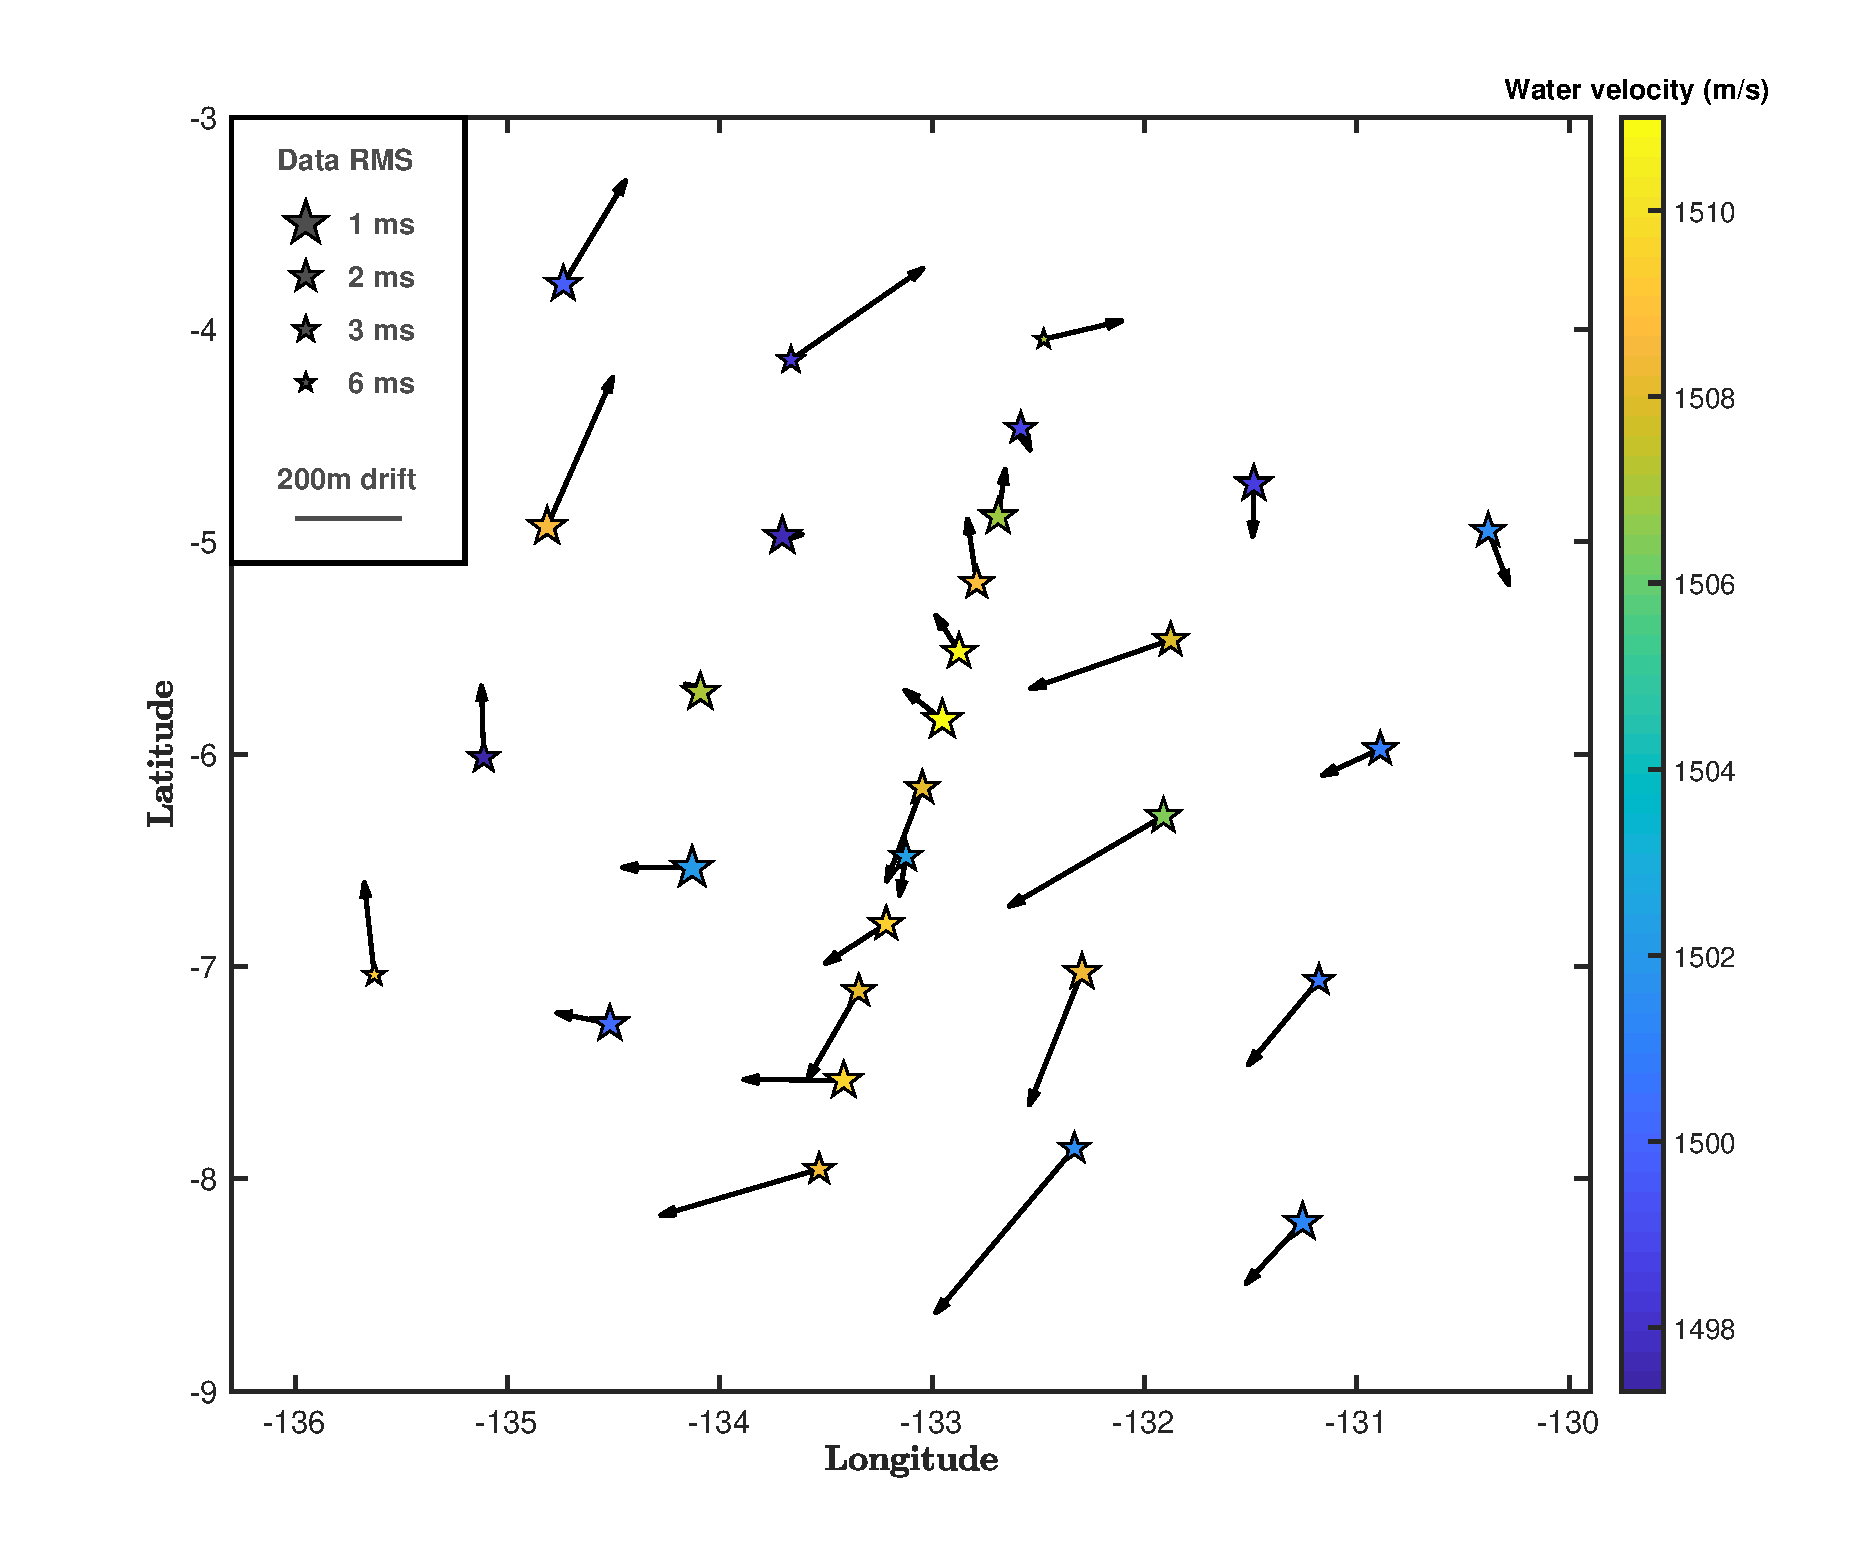
\includegraphics[trim=0cm 0cm 0cm 0cm,clip=true,width=\columnwidth]{Figure08.pdf}
%\caption{Pacific ORCA deployment, showing drift directions and magnitudes of each OBS instrument relative to their drop points, as well as the water velocity each location. Note that drift arrows are not to geographic scale. The systematic pattern of drift within the water column seems to be related to a meso-scale ocean eddy moving through this region during the deployment. Station symbol sizes are inversely scaled to acoustic travel time data misfit (see inset).}
%\label{fig:meso_eddy}
%\end{figure}

%% Comparison to previous tools
\begin{figure}[h]
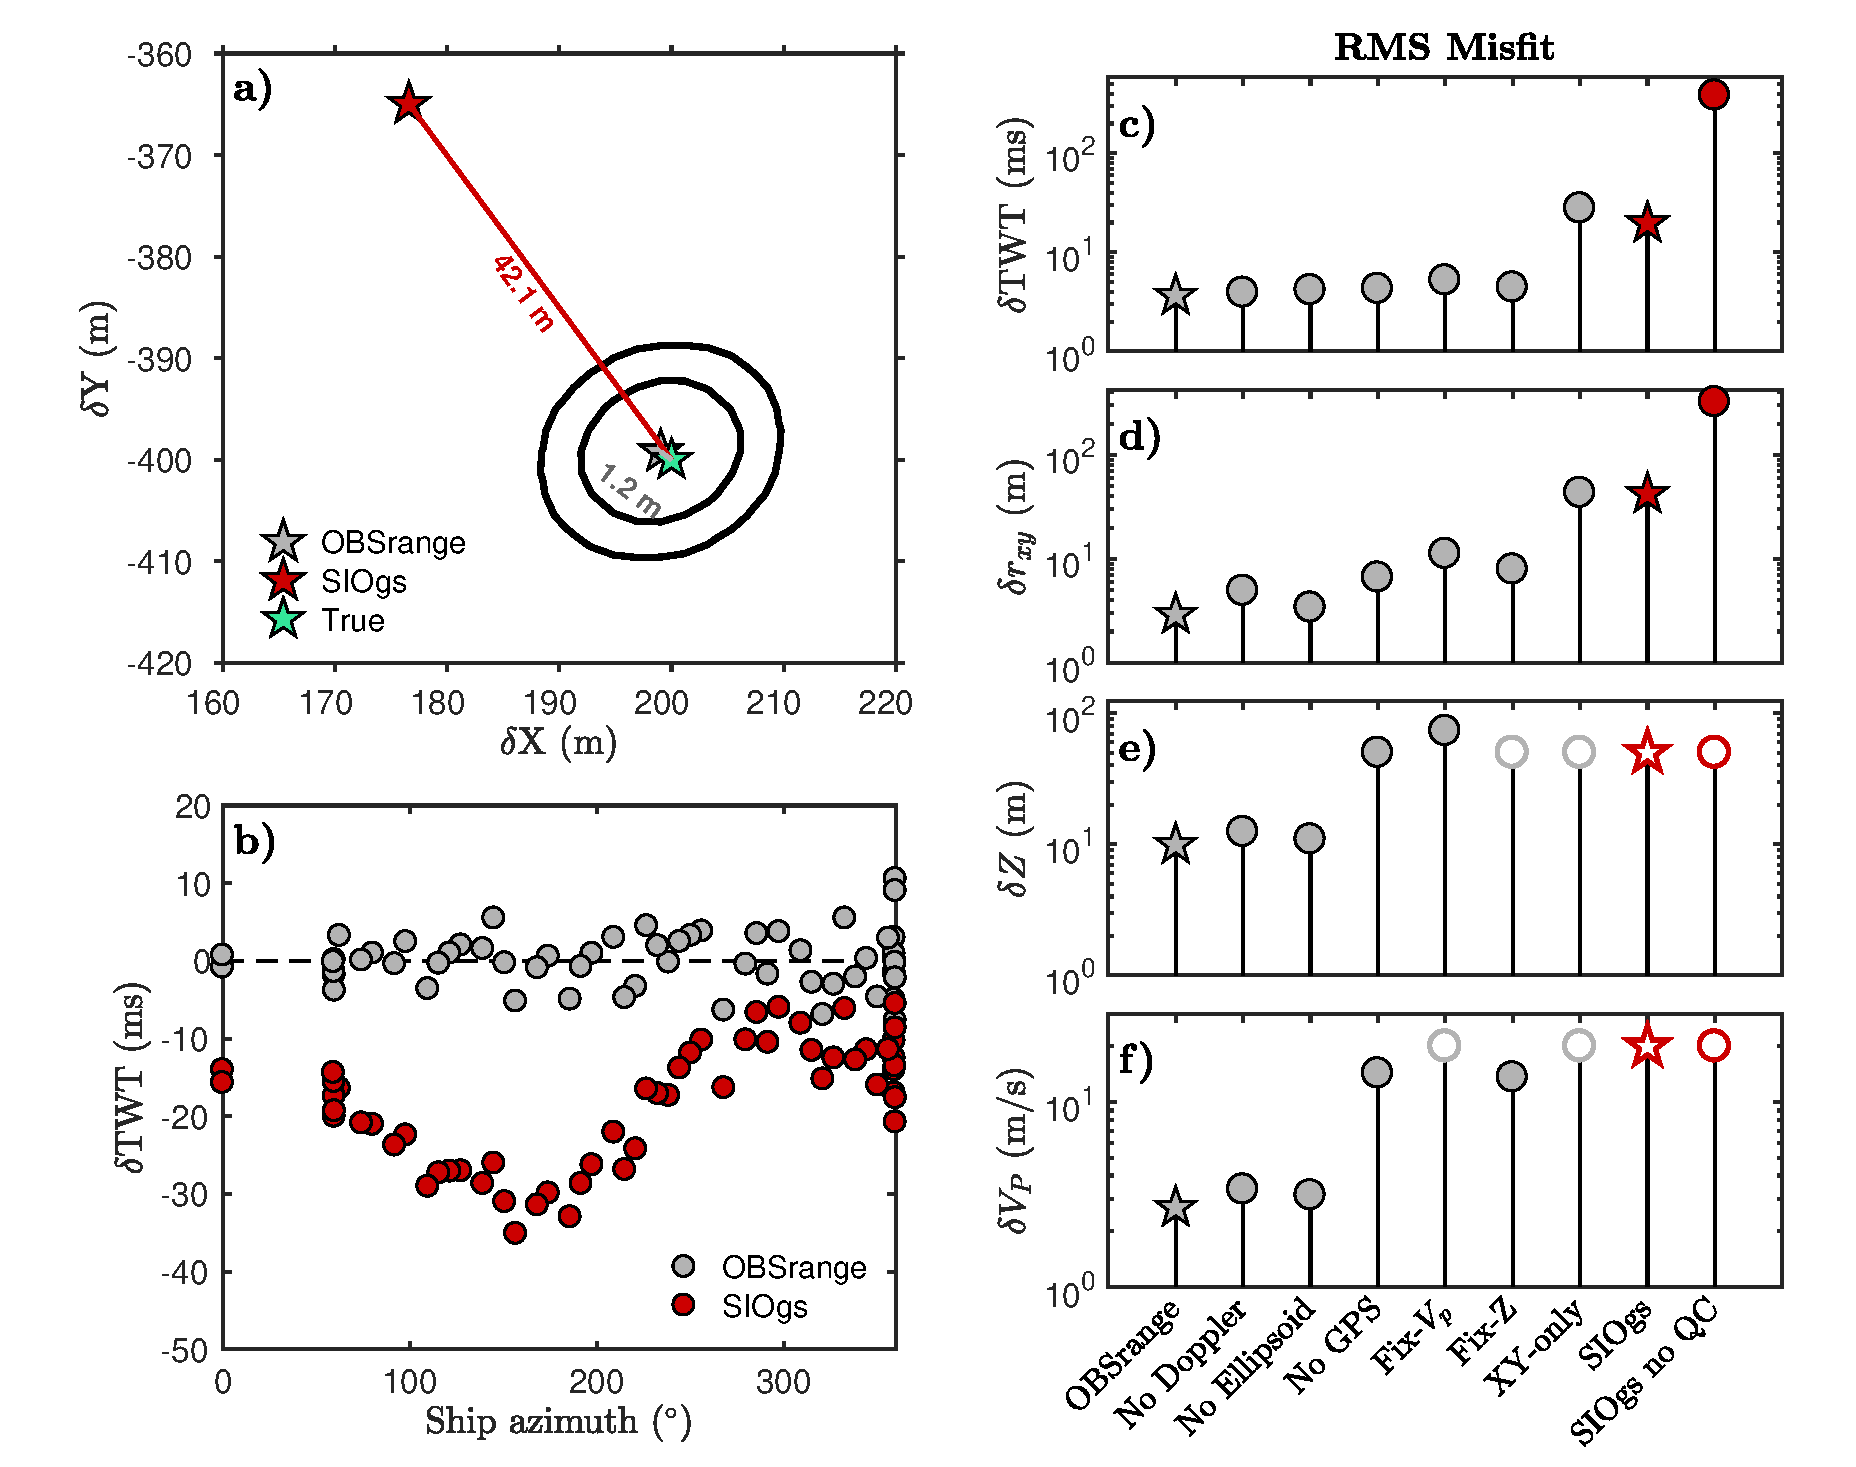
\includegraphics[trim=0cm 0cm 0cm 0cm,clip=true,width=\columnwidth]{Figure05.pdf}
\caption{ Synthetic test of OBSrange performance (gray symbols) compared with the SIO tool (red symbols) for a \textit{PACMAN} survey of radius 1 Nm. a) Map view comparing the OBSrange and SIO inverted instrument locations with the true location in green. Black contours show the 68\% and 95\% confidence from the F-test. b) Two-way time (TWT) residuals for both methods as a function of ship azimuth from the true station location. c) TWT and d--g) model parameter RMS misfits for 9 inversions, where closed symbols represent parameters that are solved for in the inversion and open symbols are parameters that remain fixed throughout the inversion. The mislocation in $x$--$y$ is given by $\delta r_{xy} = \sqrt{\delta x_{O}^2 + \delta y_{O}^2} $. Stars in c--g mark the inversions shown in a) and b). See table 1 for details of the 9 inversions.}
\label{fig:compare_tool}
\end{figure}

%% Exploring survey geometries
\begin{figure}[h]
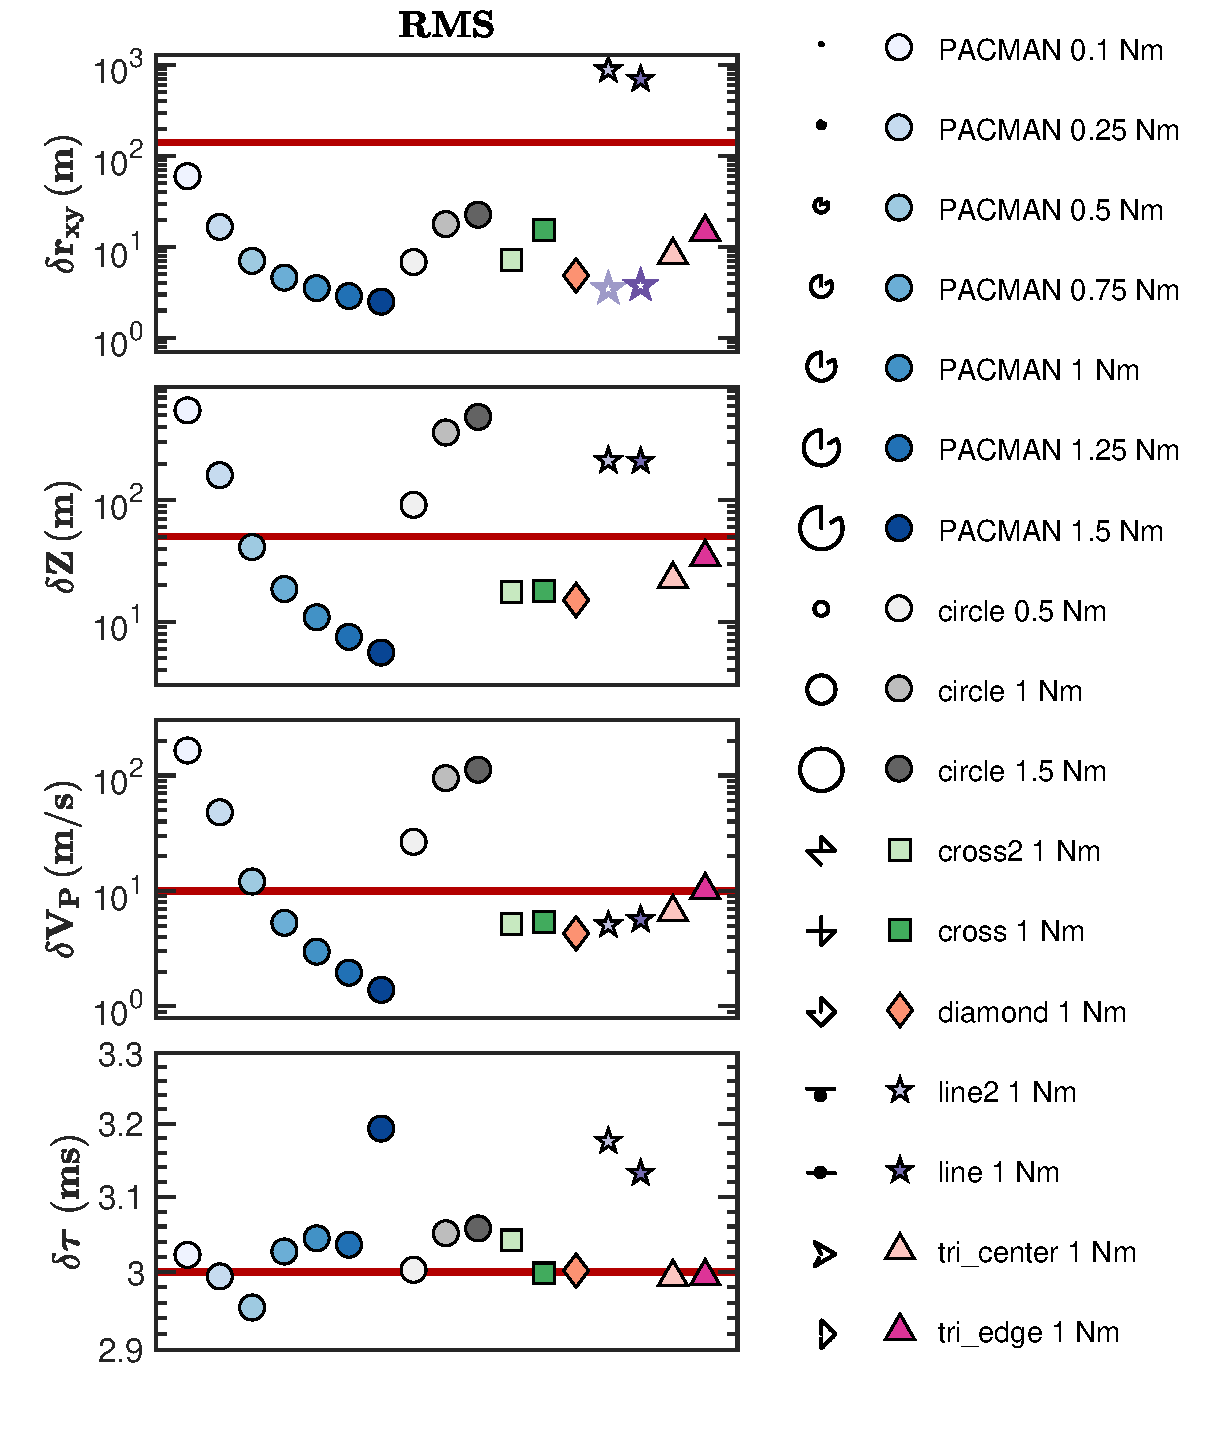
\includegraphics[trim=0cm 0cm 0cm 0cm,clip=true,width=\columnwidth]{Figure06.pdf}
\caption{ Model parameter RMS misfits for 6 synthetic survey geometries of varying radii: \textit{PACMAN}, circle, cross, diamond, line, and triangle. Each survey geometry is shown to the left of its respective legend entry. Panels show the RMS misfit for each model parameter and survey type for 10,000 synthetic survey realizations, where the mislocation in $x$--$y$ is given by $\delta r_{xy} = \sqrt{\delta x_{O}^2 + \delta y_{O}^2} $. We find that model parameters are most accurately recovered using the \textit{PACMAN} survey pattern with radius $\geq$1 Nm, and the line surveys perform worst. }
\label{fig:survey_geom_explore}
\end{figure}

